\subsection{Variational Monte Carlo calculations of the helium atom}
		As a first attempt to solve the ground state energy for the helium
		atom we perform Variational Monte Carlo calculation with a brute force
		Metropolis sampling. We do this with two trial wave functions
		\[
		\psi_{T1}({\bf r_{1}},{\bf r_{2}},{\bf r_{12}})=\exp{\left(-\alpha(r_{1}+r_{2})\right)}
		\]
		and
		\[
		\psi_{T2}({\bf r_{1}},{\bf r_{2}},{\bf r_{12}})=\exp{\left(-\alpha(r_{1}+r_{2})\right)}\exp{\left(\frac{r_{12}}{2(1+\beta r_{12})}\right)},
		\]
		using $\alpha$ and $\beta$ as variational parameters. Energy values
		for the simple wave function, $\psi_{T1}$, using only one variational
		parameter $\alpha$, are shown in figure \ref{fig01:alpha_Simple}.
		We run the Variational Monte Carlo calculation with $10^{7}$ cycles.
		As we see in the figures, the energy minimum occurs when we use $\alpha=1.65$.
		Using this value for $\alpha$ we get an energy of $-2.8442934$.
		The parameter $\alpha$ can be interpreted as a parameter for the
		force pulling the electron to the nucleus.


	\begin{figure}
	\centering 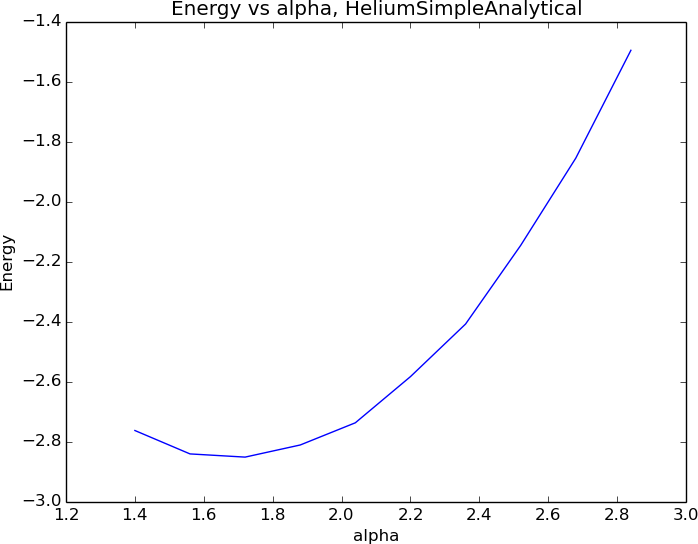
\includegraphics[width=0.45\linewidth]{../figures/EnergyVsAlphaHeliumSimpleAnalytical}
	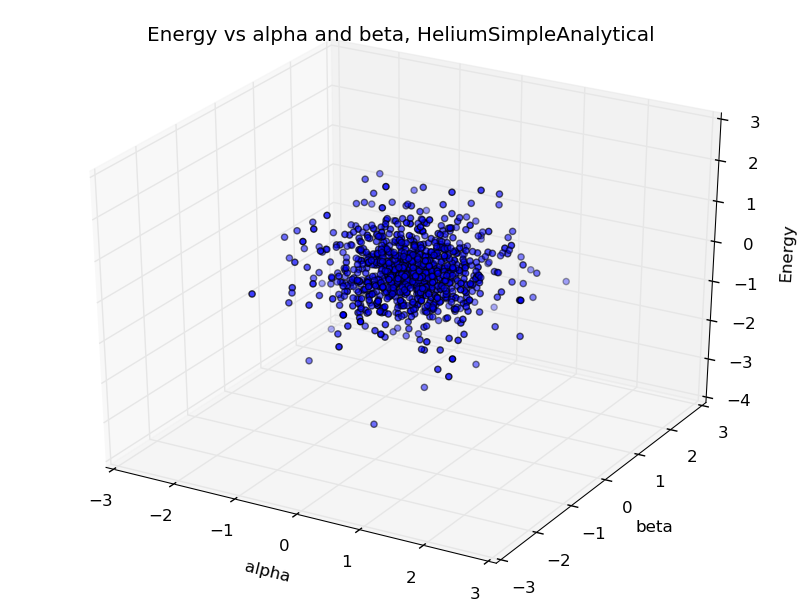
\includegraphics[width=0.45\linewidth]{../figures/VarianceVsAlphaHeliumSimpleAnalytical}

	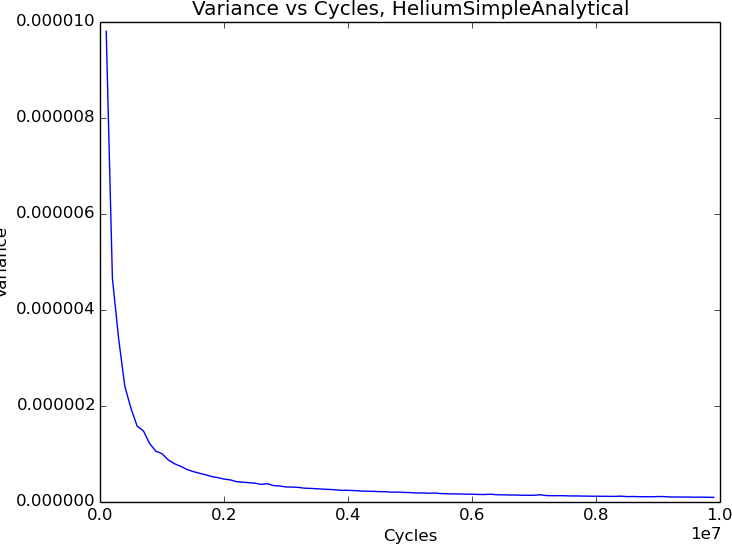
\includegraphics[width=0.45\linewidth]{../figures/VarianceNCyclesHeliumSimpleAnalytical}\protect\protect\caption{Plots for Helium $\psi_{T1}$ for energy versus $\alpha$, variance versus $\alpha$, and variance as function of Monte Carlo cycles.}
	\label{fig01:alpha_Simple}
	\end{figure}


	\begin{figure}
	\centering 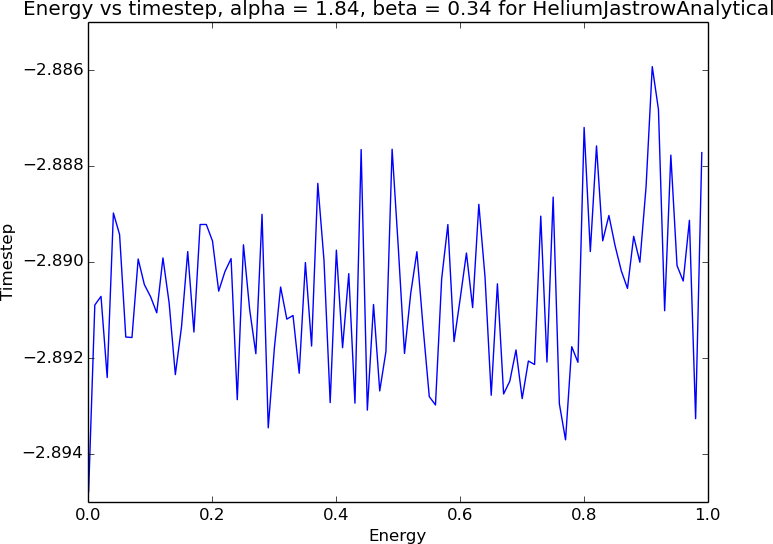
\includegraphics[width=0.45\linewidth]{../figures/HeliumJastrowAnalyticalTimeEnergy}
	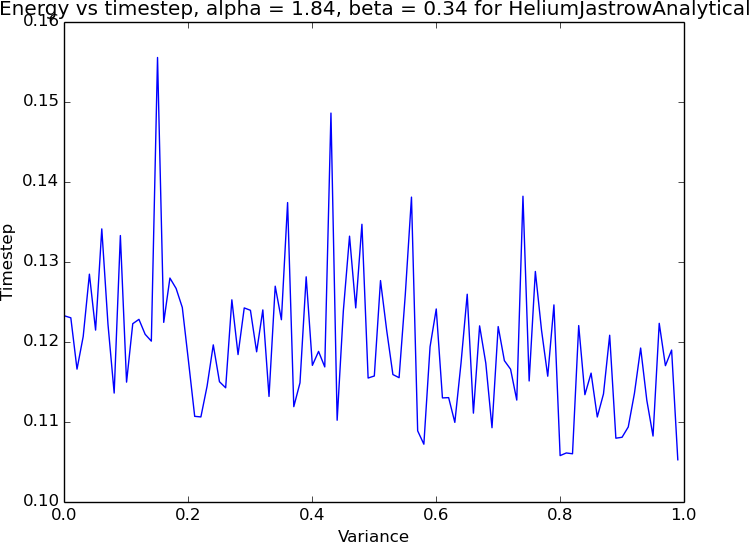
\includegraphics[width=0.45\linewidth]{../figures/HeliumJastrowAnalyticalTimeVariance}
	\protect\caption{Plots for Helium $\psi_{T2}$ for the energy versus the timestep, and the variance versus the timestep.}
	\label{fig02:timestep}
	\end{figure}

	We now look at our second trial function, $\psi_{T2}$. Running over
	different values for the two variables $\alpha$ and $\beta$, again
	with $10^{7}$ cycles in the Monte Carlo simulation, we get the results
	presented in figure \ref{fig03:AlphaBeta}. From this run we find
	that the optimal values are $\alpha=1.8$ and $\beta=0.94$, and we
	get a minimum energy of $-2.8979105$, which is considerably better
	than without the Jastrow factor.

\begin{figure}
	\centering 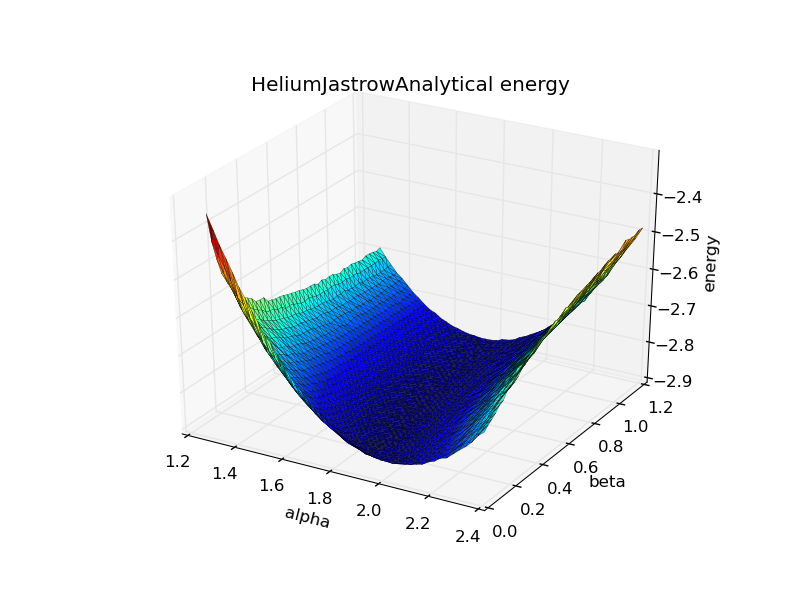
\includegraphics[width=0.45\linewidth]{../figures/HeliumJastrowAnalytical_alpha_beta_energy}
	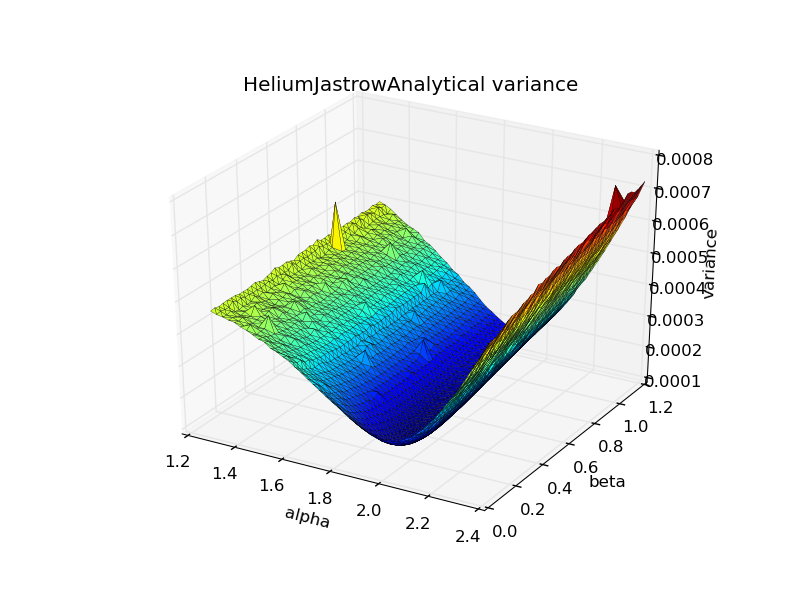
\includegraphics[width=0.45\linewidth]{../figures/HeliumJastrowAnalytical_alpha_beta_variance}
	\protect\caption{Using $\psi_{T2}$, plot of the energy versus alpha and beta, and plot of the variance versus $\alpha$ and $\beta$. }
	\label{fig03:AlphaBeta}
	\end{figure}

	Finally we use our Variational Monte Carlo machinery to find the ground
	state energy for a beryllium atom. Since beryllium has 4 electrons,
	compared to the 2 in helium, the computation is much slower and we
	only had time to run it for $10^{6}$ cycles. We then find the lowest
	energy to be $-14.4127$ with $\alpha=3.8$ and $\beta=0.293$.

	From reseach papers we find the value for energy in the ground state
	of helium to be $-2.9037$ \cite{Kinoshita:1957:PR} and the value
	for energy in the ground state of beryllium to be $-14.667$ \cite{Koput:2011:PCCP}.
	Koput{]}. In table (\ref{tab:energyReference1}) we compare results
	obtained with our Variational Monte Carlo method with results from
	various research papers.

	\begin{table}
		\centering
		\begin{tabular}{|c|c|c|}
			\hline
			Atom & VMC & References\tabularnewline
			\hline
			\hline
			Helium $\psi_{T1}$ & $-2.8442$ & $-2.9037$ \tabularnewline
			\hline
			Helium $\psi_{T2}$ & $-2.8979$ & $-2.9037$ \tabularnewline
			\hline
			Beryllium & $-14.4127$ & $-14.667$\tabularnewline
			\hline
		\end{tabular}

		\protect
		\caption{Comparison of energies found with Variational Monte Carlo method and
		energies found in research papers.}
		\label{tab:energyReference1}
	\end{table}

	\subsubsection{Alpha and Beta Values}

		\begin{table}
			\center
			\begin{tabular}{| c | c| c |}
			    \hline
			   	\textbf{Trialfunction} & \(\mathbf{\alpha}\) & \(\mathbf{\beta}\)
			    \\ \hline
			    Helium $\psi_{T1}$ & 1.65 & -
			    \\ \hline
			    Helium $\psi_{T2}$ & 1.8 & 0.94
			    \\	\hline
			    Beryllium $\psi_{T2}$	& 3.8	&	 0.293
			    \\ \hline
	  		\end{tabular}
	  		\caption{The values for \(\alpha\) and \( \beta \) where found by doing running Monte Carlo calculation with over a mesh of different \(\alpha\) and \( \beta \) values, with stepssize \(0.02\). Each Monte Carlo run went over \(10 000 	000\), using importance sampling. Then the run with the lowest energy gave the \(\alpha\) and \(\beta\) values.}
		  	\label{tab:alpha_beta1}
		\end{table}

		Table \ref{tab:alpha_beta1} shows the values, for \(\alpha\) and \(\beta\) values, we got from  running several Monte Carlo cycles with different values. As an algorithm to pick out the best values we minimized the energy found in the Monte Carlo runs. The values found are quite uncertain since the variance of the energy was quite high compared to the difference caused by varying the parameters. The variance was more smooth as a function of the parameters, see fig \ref{fig03:AlphaBeta} and should have been used.




			\subsubsection{Computational speed gain by using an analytical local energy}
				By using an analytical expression for the local energy instead of using a numerical derivation in the calculation a speed up of approximately factor \(4\) was achieved, see table \ref{tab:analyticVSNumeric}.


				\begin{table}
					\center
					\begin{tabular}{| c | c | c | c |}
					    \hline
					   	\textbf{Trialfunction} & Numerical (s) & Analytical (s) & Ratio
					    \\ \hline
					    Helium $\psi_{T1}$ & 61.75 & 14.34 & 4.307
					    \\ \hline
					    Helium $\psi_{T2}$ & 86.76 & 19.98	& 4.342
					    \\	\hline
					    Beryllium $\psi_{T2}$ & 1918.34  &	 &
	 				    \\ \hline
					\end{tabular}
					\caption{The time to run a Monte Carlo run with \(10^7\) cycles. The closed expression for the local energy increased the computation time by a significant degree for each trialfunction. }
					\label{tab:analyticVSNumeric}
				\end{table}